\section{Forward Kinematics}

In order to compute the forward kinematcs of the arm all joint axes has been fixed using the Denavit-Hartenberg conventions.

\begin{figure}[h]
\centering
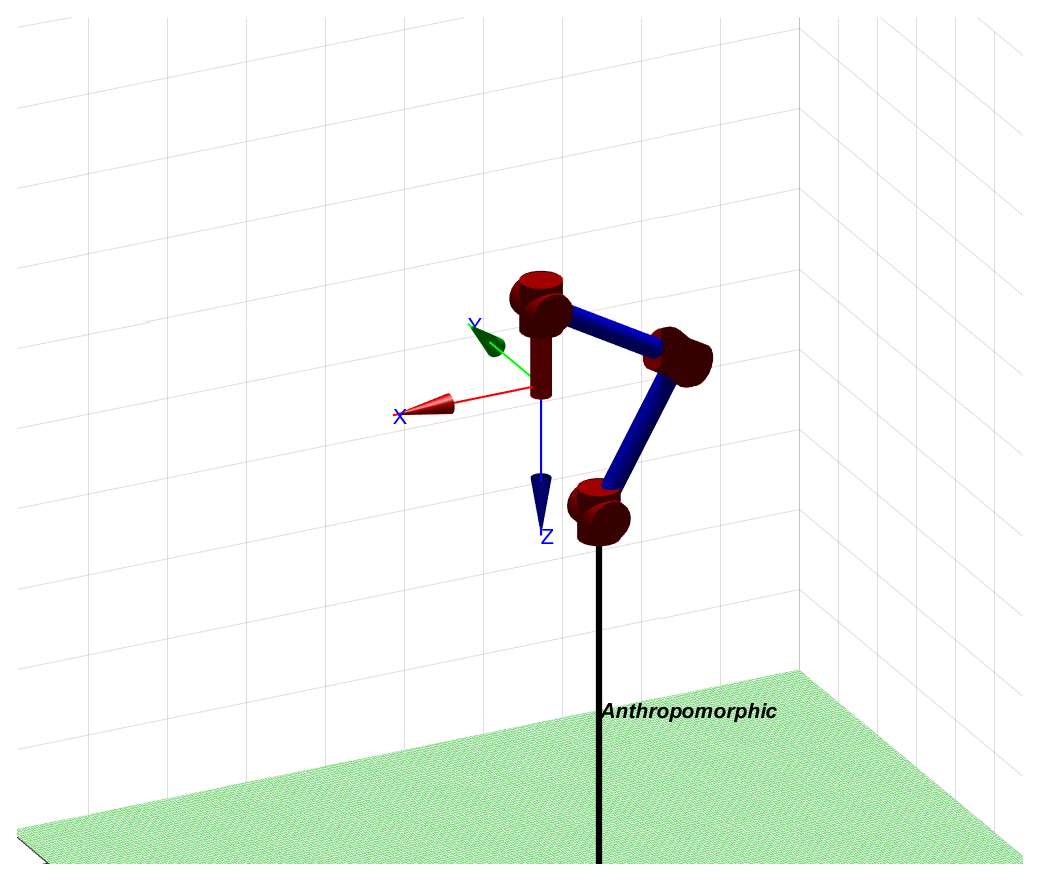
\includegraphics[width=0.8\linewidth]{img/aarm}
\caption{6 DOF Antrhopomorphic Arm}
\label{fig:aarm}
\end{figure}

Figure \ref{fig:aarm} shows the Aarm in its initial pose and Figure \ref{fig:dhtable} the respective DH-parameters, being $q_{i}$ the joint angles.

\begin{figure}[h]
\centering
\includegraphics[width=0.8\linewidth]{img/dhtable}
\caption{Denavit Hattenberg parameters}
\label{fig:dhtable}
\end{figure}

According to DH-convention, the generic homogeneous transformation converting coordinates of frame $i-1$ in coordinates of frame $i$  
is:

\vspace{1cm}
$
A^{i-1}_{i} =
\left(
\begin{matrix}
	\cos{(q_i)} & -\sin{(q_i)}\cos{(\alpha_i)} & \sin{(q_i)}\sin{(\alpha_i)}  & a_i\cos{(q_{i})} \\ 
	\sin{(q_i)} & \cos{(q_{i})}\cos{(\alpha_i)} & -\cos{(q_i)}\sin{(\alpha_i)} & a_i\sin{(q_{i})} \\ 
	0 & \sin{(\alpha_i)} & cos{(\alpha_i)} & d_i \\ 
	0 & 0  & 0  & 1
\end{matrix} 
\right)
$\newpage
computing the $i^{-th}$ transformation as:
\begin{center}
	$p_i = A^{i-1}_{i} \cdot p_{i-1}$
\end{center}
The total forward kinematics can be expressed once defined two more homogeneous matrix that represents position and orientation of base and tool frame with respect to frame 0 and frame n respectively:
\begin{center}
$T^b_e = T^b_0T^0_nT^n_e$	
\end{center}
where $T^0_n = A^0_1(q_1)A^1_2(q_2)...A^{n-1}_n$.\newline
Referring to Fig.\ref{fig:dhtable} it is possible to derive all transformation matrix for the Anthropomorphic manipulator:
\begin{center}
$A^0_1(q_1) = \left(
\begin{matrix}
\cos{(q_1)} & 0 & \sin{(q_1)} & 0 \\ 
\sin{(q_1)} & 0 & -\cos{(q_1)} & 0 \\ 
0 & 1 & 0 & 0 \\ 
0 & 0 & 0 & 1 
\end{matrix}
\right)$
\vspace{0.5cm}

$A^1_2(q_2) = \left(
\begin{matrix}
\cos{(q_2)} & -\sin{(q_2)} & 0 & a_2\cos{(q_2)} \\ 
\sin{(q_2)} & \cos{(q_2)} & 0  & a_2\sin{(q_2)} \\ 
0 & 0 & 1 & 0 \\ 
0 & 0 & 0 & 1 
\end{matrix}
\right)$
\vspace{0.5cm}

$A^2_3(q_3) = \left(
\begin{matrix}
\cos{(q_3)} & 0 & \sin{(q_3)} & 0 \\ 
\sin{(q_3)} & 0 & -\cos{(q_3)} & 0 \\ 
0 & 1 & 0 & 0 \\ 
0 & 0 & 0 & 1 
\end{matrix}
\right)$
\vspace{0.5cm}

$A^3_4(q_3) = \left(
\begin{matrix}
\cos{(q_4)} & 0 & -\sin{(q_4)} & 0 \\ 
\sin{(q_4)} & 0 & \cos{(q_4)} & 0 \\ 
0 & -1 & 0 & d_4 \\ 
0 & 0 & 0 & 1 
\end{matrix}
\right)$
\vspace{0.5cm}

$A^4_5(q_5) = \left(
\begin{matrix}
\cos{(q_5)} & 0 & \sin{(q_5)} & 0 \\ 
\sin{(q_5)} & 0 & -\cos{(q_5)} & 0 \\ 
0 & 1 & 0 & 0 \\ 
0 & 0 & 0 & 1 
\end{matrix}
\right)$
\vspace{0.5cm}

$A^5_6(q_6) = \left(
\begin{matrix}
\cos{(q_6)} & -\sin{(q_6)} & 0 & 0 \\ 
\sin{(q_6)} & \cos{(q_6)} & 0 & 0 \\ 
0 & 0 & 1 & d_6 \\ 
0 & 0 & 0 & 1 
\end{matrix}
\right)$
\end{center}
